\documentclass[border=2pt]{standalone}
\usepackage{pgfplots}
\usepgfplotslibrary{statistics}
\pgfplotsset{compat=1.18}
\begin{document}
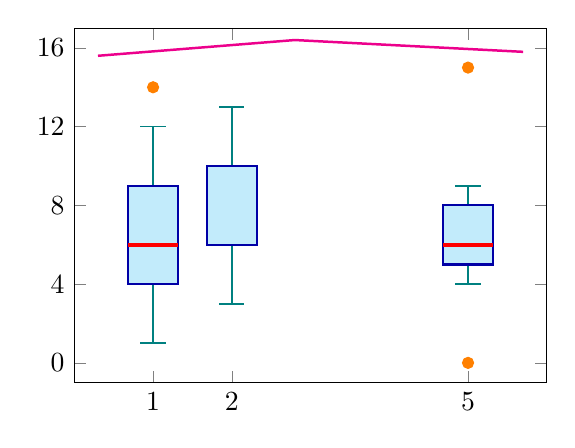
\begin{tikzpicture}
\begin{axis}[
    width=60mm,height=45mm,scale only axis,
    xmin=0,xmax=6,ymin=-1,ymax=17,xtick={1,2,5},ytick={0,4,8,12,16},
    boxplot/draw direction=y,boxplot/box extend=0.64,boxplot/whisker extend=0.32,
    boxplot/every box/.style={fill=cyan!24,draw=blue!65!black,line width=0.8pt},
    boxplot/every whisker/.style={draw=teal,line width=0.6pt},
    boxplot/every median/.style={draw=red,line width=1.4pt},
]
    \addplot[orange,mark=*,mark size=2pt,boxplot prepared={
        lower whisker=1,lower quartile=4,median=6,upper quartile=9,upper whisker=12,
    }] coordinates {(3,14)};
    \addplot[magenta,no marks,line width=0.9pt] coordinates {(0.3,15.6) (2.8,16.4) (5.7,15.8)};
    \addplot[orange,boxplot prepared={
        lower whisker=3,lower quartile=6,upper quartile=10,upper whisker=13,
    }] coordinates {};
    \addplot[orange,mark=*,mark size=2pt,boxplot={draw position=5}]
        coordinates {(4,8) (2,0) (3,5) (0,15) (4,6) (1,9) (3,4) (2,7) (1,5)};
\end{axis}
\end{tikzpicture}
\end{document}
